Este capítulo apresenta os resultados obtidos com o desenvolvimento do sistema web, e com as consultas feitas tanto para obter informações relevantes sobre a CEAP, quanto para detectar possíveis fraudes.

\section{Consultas CEAP - TSE} \label{consulta_ceap_tse}

A partir da tela inicial apresentada na Figura \ref{fig:sistema_ceap}, é possível navegar para as demais telas utilizando a barra azul de navegação. Nessa barra de navegação ao clicar no link "CEAP / TSE", o sistema redireciona o usuário para uma tela que fornece informações gerais a respeito do conjunto de dados utilizado. A Figura \ref{fig:sistema_ceap_tse} mostra a parte inicial da tela "CEAP / TSE".

\begin{figure}[H]
\centering
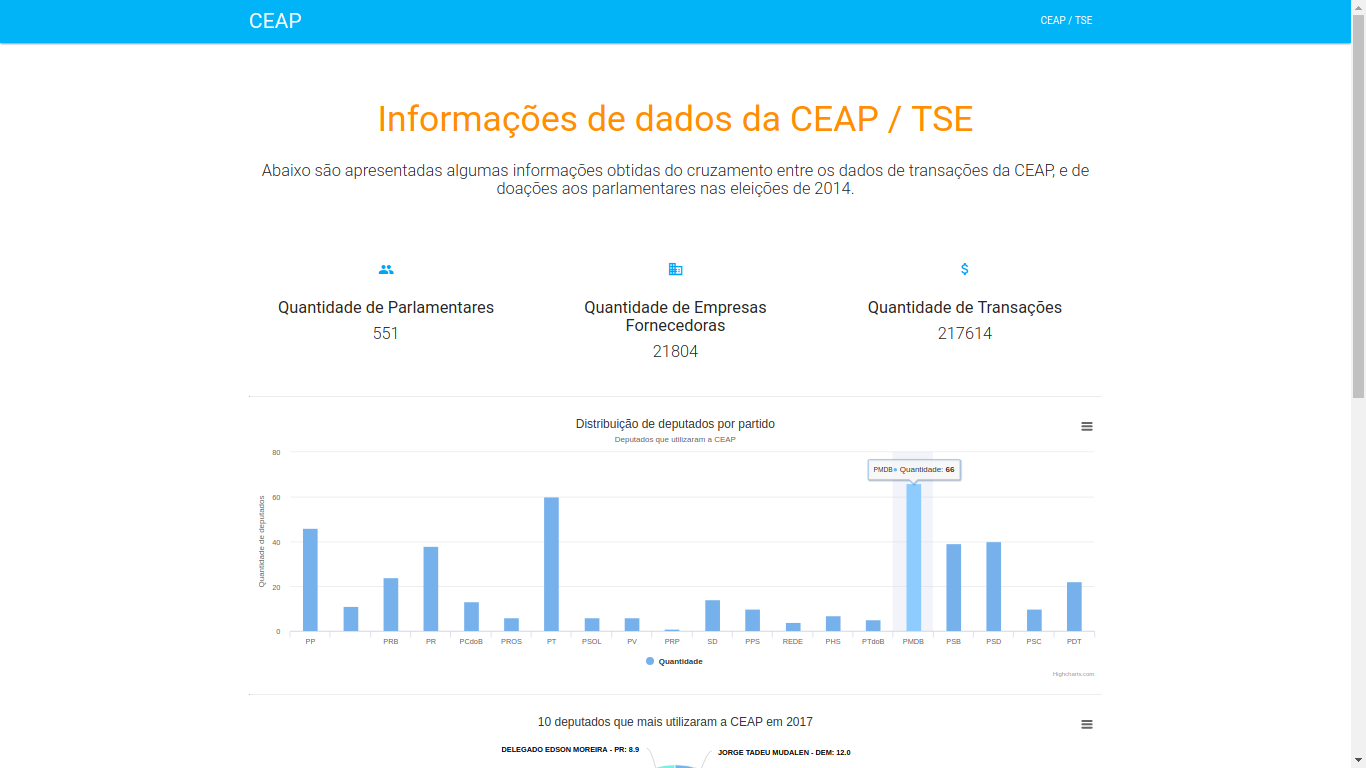
\includegraphics[width=.75\textwidth]{ceap-tse.png}
\caption{Tela de Informações Gerais do Sistema "CEAP Colaborativo".}
\label{fig:sistema_ceap_tse}
\end{figure}

No início da tela é informado que foram armazenados no banco de dados um total de 551 parlamentares, 21.804 empresas fornecedoras e 217.614 transações.
A primeira consulta feita nesta tela foi a distribuição de Deputados que utilizaram a CEAP por partido. A Figura \ref{fig:chart_1} apresenta o resultado.

\begin{figure}[H]
\centering
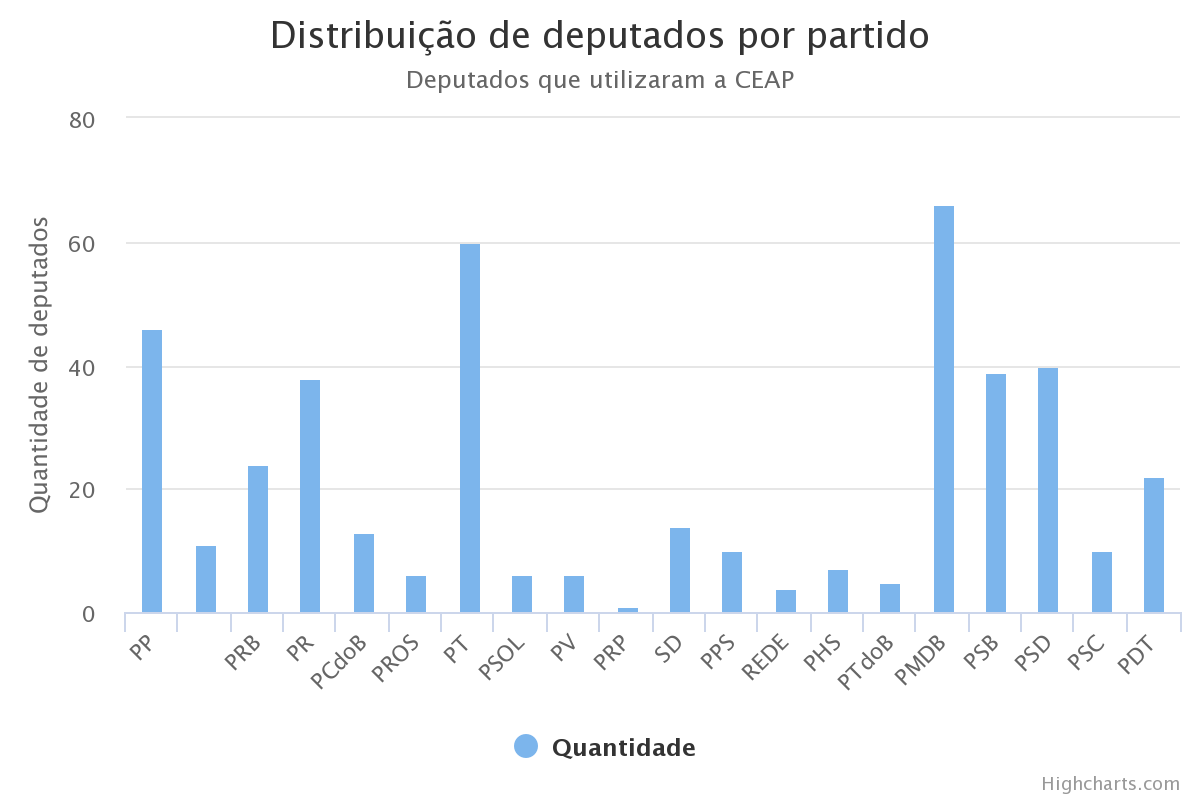
\includegraphics[width=.75\textwidth]{chart_1.png}
\caption{Distribuição de Deputados que Utilizaram a CEAP por Partido.}
\label{fig:chart_1}
\end{figure}

\begin{lstlisting}[label={lst:consulta_chart_1}, caption={Consulta para a Figura \ref{fig:chart_1}},captionpos=b, language=sql]
select SgPartido, count(SgPartido) from Parlamentar GROUP BY SgPartido
\end{lstlisting}

A partir da Figura \ref{fig:chart_1} é possível observar que o partido que tem mais deputados que utilizaram a CEAP no ano de 2017 foi o PMDB com 66 Deputados, seguido pelo PT com 60 Deputados, e pelo PP com 46 Deputados. É interessante notar como o OrientDB, mesmo sendo um SGBD NoSQL, possui uma linguagem baseada na linguagem de consulta SQL e, portanto, o Código \ref{lst:consulta_chart_1} se assemelha bastante a uma consulta SQL de um SGBD relacional.

A próxima consulta feita foi para obter os 10 Deputados que mais fizeram transações no ano de 2017. A Figura \ref{fig:chart_2} apresenta o resultado.

\begin{figure}[H]
\centering
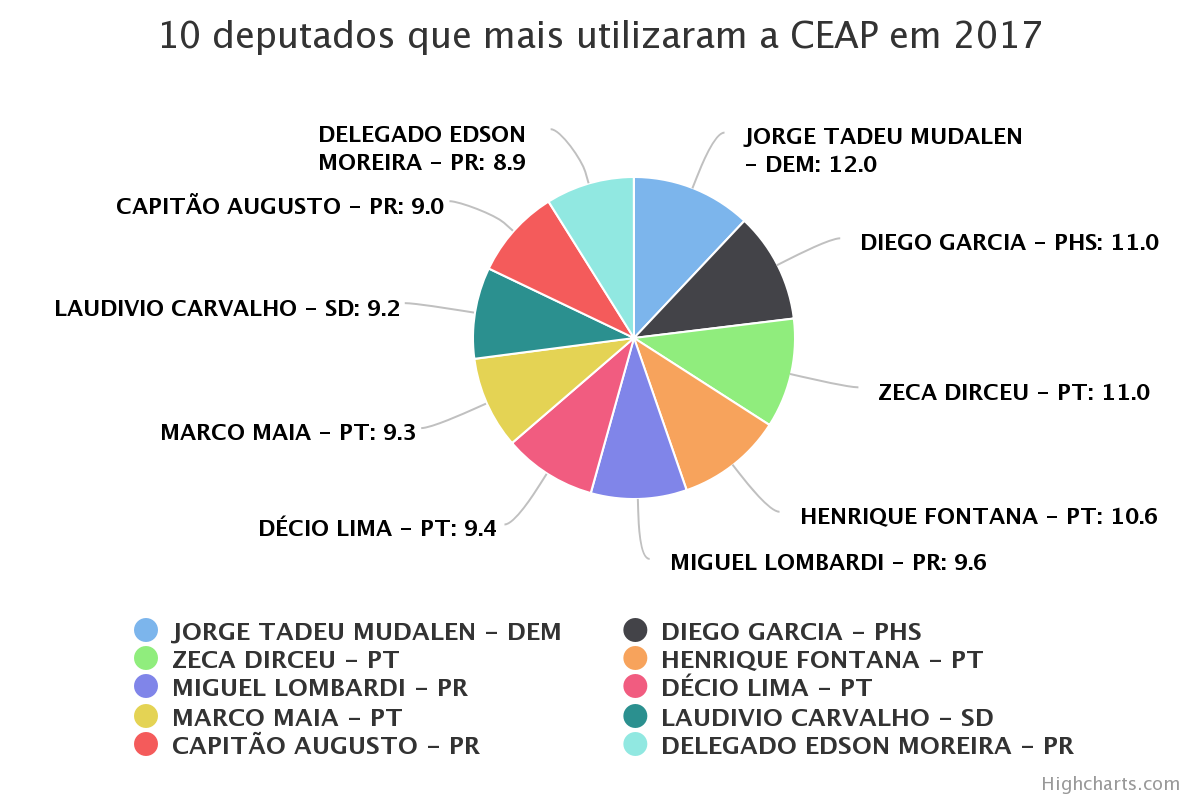
\includegraphics[width=.75\textwidth]{chart_2.png}
\caption{10 Deputados que mais Fizeram Transações no ano de 2017.}
\label{fig:chart_2}
\end{figure}

\begin{lstlisting}[label={lst:consulta_chart_2}, caption={Consulta para o gráfico \ref{fig:chart_2}},captionpos=b, language=sql]
select TxNomeParlamentar, SgPartido, out("RealizaTransacao").size() 
as transacoes from Parlamentar 
order by transacoes desc limit 10
\end{lstlisting}

Por meio da Figura \ref{fig:chart_2}, percebe-se que o Deputado que mais realizou transações foi o Jorge Tadeu Mudalen do partido DEM com 1.280 transações, seguido pelo Diego Garcia do PHS com 1.176 transações, e pelo Zeca Dirceu do PT com 1.173 transações. O Código \ref{lst:consulta_chart_2} por sua vez, possui elementos específicos do OrientDB, que no caso é a função "out". Nessa consulta são selecionados o nome do parlamentar, o partido do parlamentar e a quantidade de arestas de classe "RealizaTransacao"\ saindo do parlamentar. Essa consulta é ordenada de forma decrescente pela quantidade de arestas que saem de um parlamentar, e limitada para obter os 10 primeiros.

A próxima consulta feita foi feita para obter as 15 empresas que mais forneceram serviços aos Deputados em 2017. A Figura \ref{fig:chart_3} apresenta o resultado.

\begin{figure}[H]
\centering
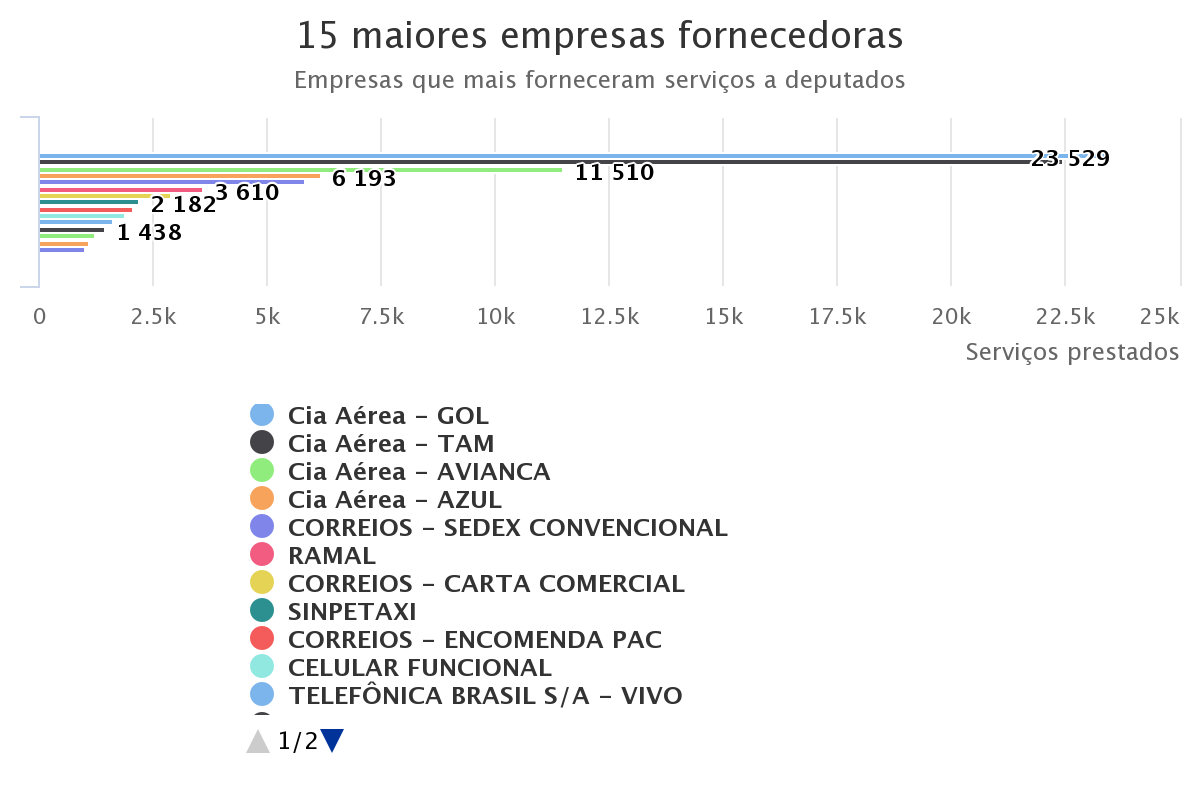
\includegraphics[width=.75\textwidth]{chart_3.png}
\caption{15 Empresas Fornecedoras que Mais Forneceram Serviços aos Deputados em 2017}
\label{fig:chart_3}
\end{figure}

\begin{lstlisting}[label={lst:consulta_chart_3}, caption={Consulta para a Figura \ref{fig:chart_3}},captionpos=b, language=sql]
select TxtFornecedor, in("FornecidaPor").size() as servicos 
from EmpresaFornecedora 
order by servicos desc limit 15
\end{lstlisting}

A partir da Figura \ref{fig:chart_3} percebe-se que as quatro primeiras empresas que mais forneceram serviços com a verba da CEAP são do ramo de aviação. Um dos propósitos da CEAP é justamente para a compra de passagens de avião, principalmente, entre Deputados de outros estados que não sejam o Distrito Federal. A Cia Aérea GOL lidera essa estatística com um total de 23.529 transações. O Código \ref{lst:consulta_chart_3} também possui elementos específicos do OrientDB, agora no caso a função "in". Nessa consulta são selecionados da classe "EmpresaFornecedora", o nome do fornecedor e a quantidade de arestas de classe "FornecidaPor"\ que entram no vértice. Em seguida, é ordenada de forma decrescente pela quantidade de arestas mencionada, e limitada para obter as 15 primeiras empresas.

Finalmente, a última consulta busca identificar no formato de um grafo parlamentares que usaram a CEAP com empresas que fizeram doações para a campanha desse parlamentar em 2014. Esse resultado foi mostrado no formato de grafo na Figura \ref{fig:ceap_tse_graph}, mas esse resultado utiliza a ferramenta gráfica presente no OrientDB. Nesse caso, a consulta foi feita e a partir do \textit{JSON}, construído um grafo na camada de apresentação do sistema desenvolvido. A Figura \ref{fig:sigma} apresenta o resultado.

\begin{figure}[H]
\centering
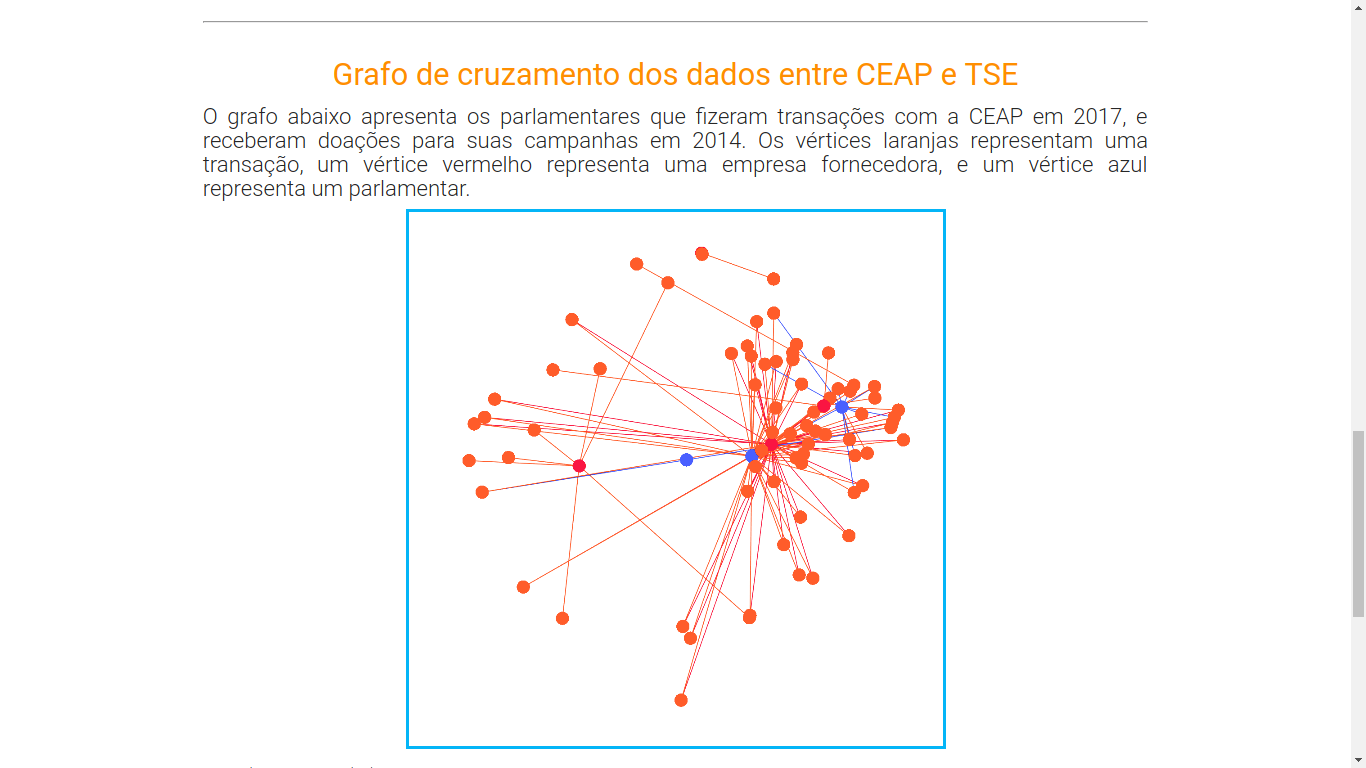
\includegraphics[width=.75\textwidth]{sigma.png}
\caption{Grafo na Camada de Apresentação com Dados do Cruzamento entre as Bases da CEAP e do TSE.}
\label{fig:sigma}
\end{figure}

O grafo utilizado na camada de apresentação possui algumas limitações, e não é robusto como o grafo apresentado pelo OrientDB. De ambas as formas foi possível encontrar o seguinte relacionamento entre os Deputados e as Empresas fornecedoras, como mostra a Tabela \ref{table:relation_deputies_companies}.

\begin{table}[h!]
\centering
\caption{Relacionamento entre Deputados e Empresas Fornecedoras.}
\begin{tabular}{|l|l|l|l|l|}
\hline
Deputado & Empresa Fornecedora \\ \hline
AELTON FREITAS & Auto Posto Cortez Ltda \\ \hline
DIEGO ANDRADE & Grafica Mundial LTDA-ME \\ \hline
MARCELO ARO & SEMPRE EDITORA LTDA. \\ \hline
WELITON PRADO & SEMPRE EDITORA LTDA. \\ \hline
TONINHO PINHEIRO & SEMPRE EDITORA LTDA. \\ \hline
MARCUS PESTANA & SOLAR COMUNICAÇÕES S.A \\ \hline
EROS BIONDINI & TARGET RENT A CAR LTDA \\ \hline
\end{tabular}
\label{table:relation_deputies_companies}
\end{table}

\section{Consultas CEAP para Detectar Fraudes}

O "CEAP Colaborativo"\ tem com um dos objetivos permitir que a população contribua com informações que possam ajudar na detecção de fraudes da CEAP. Tais informações podem ser em relação a parentes dos Deputados, e quadros de sócios das empresas fornecedoras. Portanto, ao clicar no link "Colabore"\ na tela inicial, o usuário é redirecionado para uma tela com formulários que permitem que as informações sejam submetidas. A Figura \ref{fig:collaborate} apresenta a tela em questão.

\begin{figure}[H]
\centering
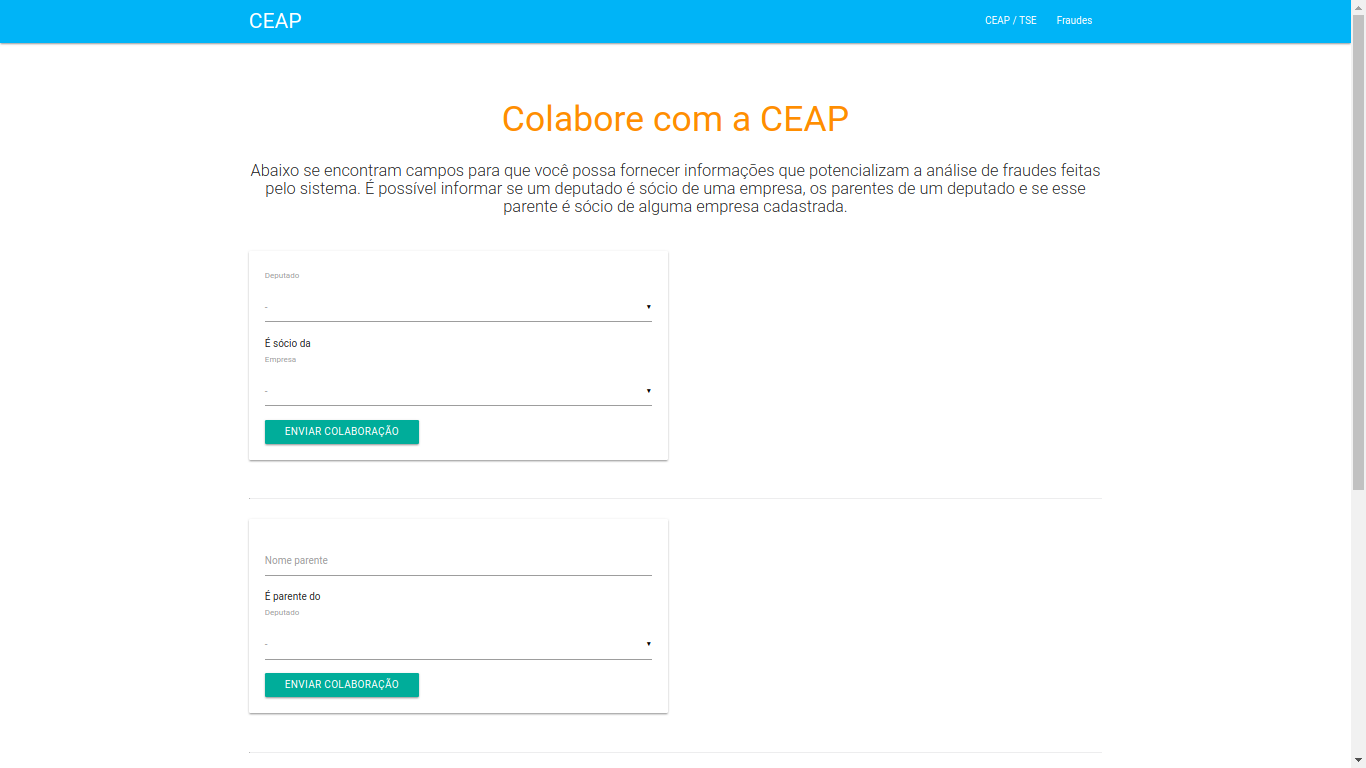
\includegraphics[width=.75\textwidth]{collaborate.png}
\caption{Tela que Permite a População Contribuir com Informações Sobre os Deputados.}
\label{fig:collaborate}
\end{figure}

Ao fornecer os dados, não é feita a persistência no OrientDB imediatamente, as informações fornecidas são salvas no SGBD relacional PostrgreSQL. Usuários administradores precisam analisar se a informação fornecida é verídica. Após essa verificação, o dado pode ser aceito ou rejeitado, e caso seja aceito é feita a persistência no OrientDB. Nessa tela é possível informar se um Deputado é sócio de uma empresa, se um deputado é parente de uma pessoa, e se algum dos parentes já cadastrados são sócios de alguma empresa cadastrada. Com essas informações, caso seja uma informação verídica, as consultas apresentadas nesta monografia irão detectar caso um padrão de fraude seja construído, e fornece os resultados nas demais telas apresentadas.

Ao clicar no \textit{link} fraudes, o sistema redireciona o usuário para uma tela que contém consultas com o objetivo de encontrar padrões que violam as regras da CEAP. Para fins de validação, foram utilizados dados fictícios para testar as consultas realizadas. A primeira análise apresentada, refere-se ao Código \ref{fig:socios} que consegue localizar um padrão de transações efetuadas entre um Deputado e uma empresa, na qual o Deputado faz parte do quadro de sócios. A Figura \ref{fig:partner} apresenta os resultados.

\begin{figure}[H]
\centering
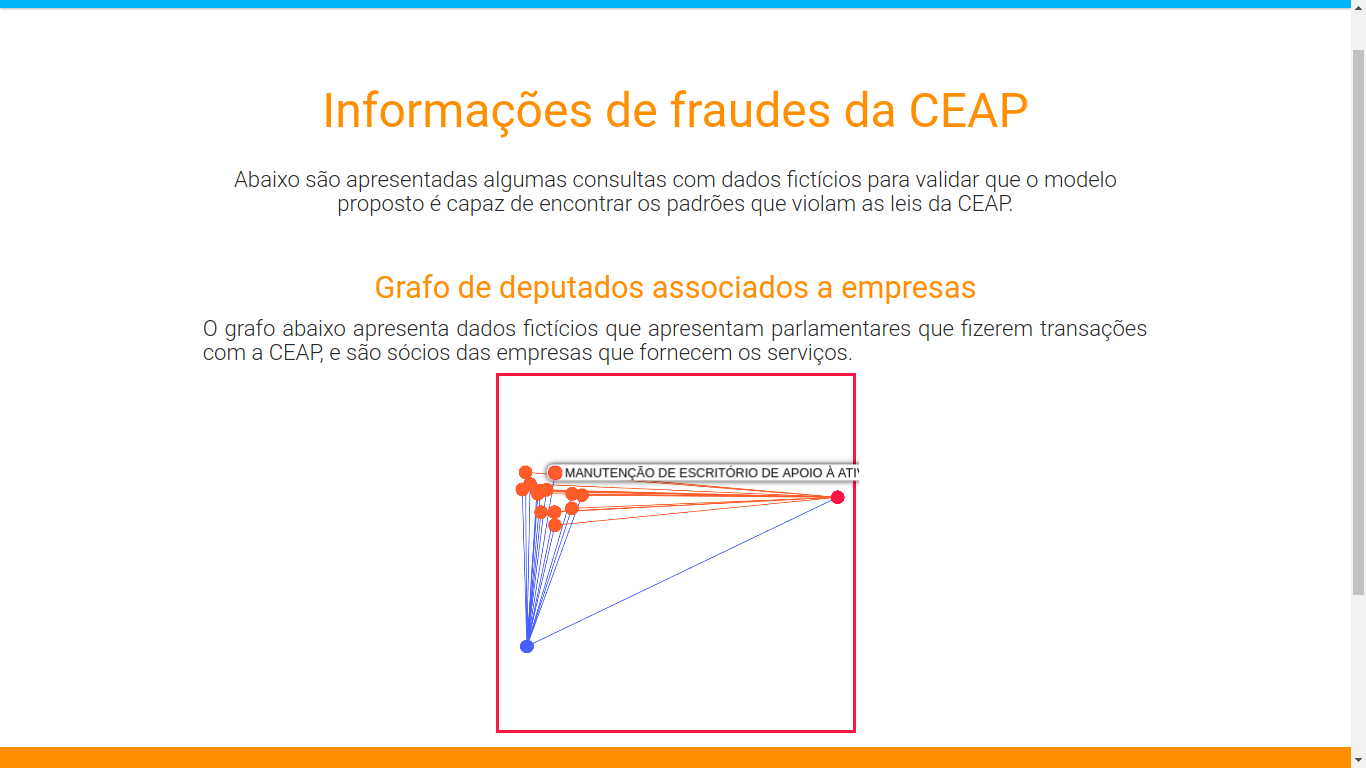
\includegraphics[width=.75\textwidth]{partner.png}
\caption{Grafo na Camada de Apresentação com Padrão de Fraude Apresentado na Figura \ref{fig:socios}.}
\label{fig:partner}
\end{figure}

A Figura \ref{fig:partner} mostra um Deputado apresentado pelo vértice em azul, que realizou transações representadas pelos vértices laranjas, fornecidas pela empresa representada pelo vértice em vermelho. Entretanto, o Deputado está relacionado com a empresa o que caracteriza uma fraude. Dessa forma, esse grafo confirma que a modelagem proposta nesta monografia é capaz de identificar indícios de fraudes nos dados da CEAP. Diferente do que foi feito na Figura \ref{fig:sigma}, não será apresentado uma tabela com o relacionamento entre um deputado e a empresa, uma vez que esse relacionamento foi criado para validar o modelo proposto.

Por fim, foi feita uma consulta que busca transações feitas com a CEAP para empresas na qual parentes do Deputado fazem parte do quadro societário. Esse padrão foi apresentado na Figura \ref{fig:familia_socio}. A Figura \ref{fig:familia_grafo} apresenta o mesmo padrão, mas feito na camada de apresentação.

\begin{figure}[H]
\centering
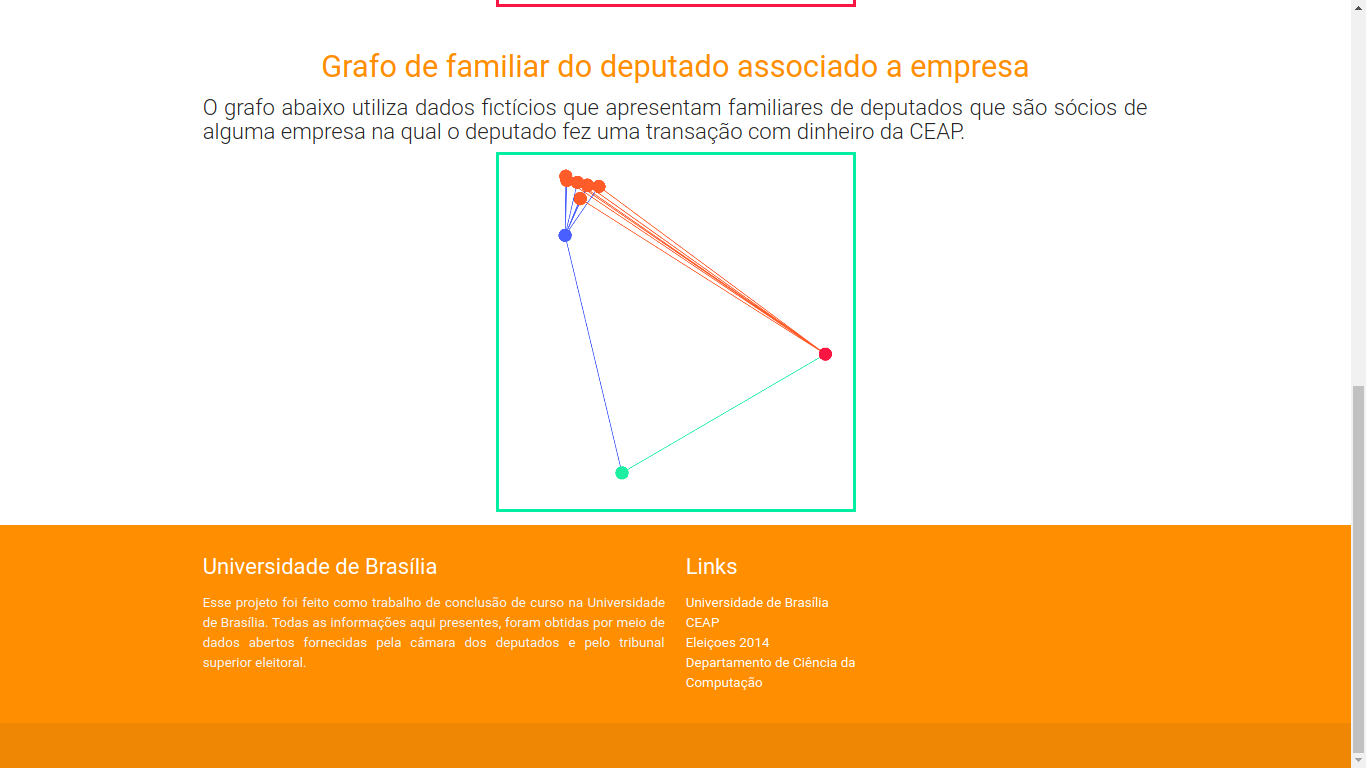
\includegraphics[width=.75\textwidth]{familia.png}
\caption{Grafo na Camada de Apresentação com Padrão de Fraude Apresentado na Figura \ref{fig:familia_socio}.}
\label{fig:familia_grafo}
\end{figure}

Dessa forma, é possível perceber que um parlamentar representado em azul é parente de uma pessoa apresentada em verde, e essa pessoa é sócia de uma empresa apresentada em vermelho. Entretanto, o parlamentar fez transações com a CEAP fornecidas pela empresa o que caracteriza fraude. Novamente, esse grafo confirma que a modelagem proposta nesta monografia é capaz de identificar fraudes nos dados da CEAP. 